% !TEX root = ../../../main.tex

\toggletrue{image}
\toggletrue{imagehover}
\chapterimage{binary_heart}
\chapterimagetitle{\uppercase{Binary Heart}}
\chapterimageurl{https://xkcd.com/99/}
\chapterimagehover{i love you}

\chapter{Schriftliche Addition von Dualzahlen}
\label{chapter-schriftliche-addition-dualzahlen}

Wir zeigen in diesem Kapitel, wie wir zwei Dualzahlen schriftlich addieren. Das Lernziel lautet:\\

\newcommand{\schriftlicheAdditionDualzahlenLernziele}{
\protect\begin{minipage}{\textwidth}
\begin{todolist}
\item Sie addieren zwei mehrstellige Dualzahlen schriftlich.
\end{todolist}
\end{minipage}
}

\lernziel{\autoref{chapter-schriftliche-addition-dualzahlen}, \nameref{chapter-schriftliche-addition-dualzahlen}}{\protect\schriftlicheAdditionDualzahlenLernziele}

\schriftlicheAdditionDualzahlenLernziele

\section{Verfahren}

Wir erinnern uns zunächst daran, wie wir das schriftliche Addieren von zwei Dezimalzahlen erlernt haben (\autoref{example-addition-dezimalzahlen}). Dazu addieren spaltenweise von rechts nach links und beachten die Überträge.

\begin{figure}[htb]
\centering
\begin{minipage}{0.45\textwidth}
\centering
\begin{example}
\label{example-addition-dezimalzahlen}
Wir addieren die Zahlen \num{1025} und \num{23987} schriftlich.
\begin{equation*}
\begin{tikzpicture}[
    row 3/.style={font=\scriptsize},
    every node/.style={column sep=.5mm, row sep=1mm}]
    \matrix (m) [matrix of math nodes,
        nodes in empty cells,
        %nodes=draw
    ] 
    {
    		& 	& 1 & 0 & 2 & 5 & [5mm]	\text{1. Summand} \\
	+      	& 2	& 3 & 9 & 8 & 7 &      \text{2. Summand} \\ 
		& 0 	& 1 & 1 & 1 &  &         \text{Überträge} \\
        		& 2 	& 5 & 0 & 1 & 2 &       \text{Summe} \\                                                  
    };

    \draw[-,color=black, semithick] (m-3-1.south west) -- (m-3-6.south east);

\end{tikzpicture}
\end{equation*}
\vspace{-0.5cm}
\end{example}
\end{minipage}
\hfill\vline\hfill
\begin{minipage}{0.45\textwidth}
\centering
\begin{example}
\label{example-addition-dualzahlen}
Wir addieren die Dualzahlen $1011_2$ und $110_2$ schriftlich.
\begin{equation*}
\begin{tikzpicture}[
    row 3/.style={font=\scriptsize},
    every node/.style={column sep=.5mm, row sep=1mm}]
    \matrix (m) [matrix of math nodes,
        nodes in empty cells,
        %nodes=draw
    ] 
    {
    		& 	& 1 & 0 & 1 & 1 & [5mm]	\text{1. Summand} \\
	+      & 	&    & 1 & 1 & 0 &      	\text{2. Summand} \\ 
		& 1 	& 1 & 1 & 0 &    &         	\text{Überträge} \\
        		& 1 	& 0 & 0 & 0 & 1 &      	 \text{Summe} \\                                                  
    };
    \draw[-,color=black, semithick] (m-3-1.south west) -- (m-3-6.south east);
\end{tikzpicture}
\end{equation*}
\vspace{-0.5cm}
\end{example}
\end{minipage}
\end{figure}

Für die schriftliche Addition von zwei Dualzahlen müssen wir verstehen, wie zwei Binärziffern addiert werden. Es gibt vier Möglichkeiten, um zwei Binärziffern zu addieren:

\begin{figure}[ht]
\centering
\begin{minipage}{0.2\textwidth}
\centering
\begin{tblr}{ccc}
  & & 0 \\
+ & &0 \\
 & {\scriptsize 0} & \\
\hline
 & & 0 \\
\end{tblr}
\end{minipage}
\begin{minipage}{0.2\textwidth}
\centering
\begin{tblr}{ccc}
  & & 0 \\
+ & &1 \\
 & {\scriptsize 0} & \\
\hline
 & & 1 \\
\end{tblr}
\end{minipage}
\begin{minipage}{0.2\textwidth}
\centering
\begin{tblr}{ccc}
  & & 1 \\
+ & &0 \\
 & {\scriptsize 0} & \\
\hline
 & & 1 \\
\end{tblr}
\end{minipage}
\begin{minipage}{0.2\textwidth}
\centering
\begin{tblr}{ccc}
  & & 1 \\
+ & &1 \\
 & {\scriptsize 1} & \\
\hline
 & & 0 \\
\end{tblr}
\end{minipage}
\end{figure}

\vspace{-0.5cm}

Bei der Addition von \textbf{zwei Einsen} erfolgt ein Übertrag von \num{1} sonst \num{0}. 

\begin{important}
Mehrstellige Dualzahlen werden nun (wie im Dezimalsystem auch) von rechts nach links addiert. Spalte für Spalte werden die Binärziffern addiert und der Übertrag beachtet.
\end{important}

In \autoref{example-addition-dualzahlen} wird eine vierstellige Dualzahl und eine dreistellige Dualzahl addiert.

\begin{important}
Falls \textbf{drei} Einsen addiert werden müssen (dies kann durch einen Übertrag passieren), dann ergibt dies in der Summe \num{1} und im Übertrag auch eine \num{1}.	
\end{important}

\vspace{-0.5cm}

\section{Übungen}

\begin{exercise}
\begin{enumerate}
\item Addieren Sie schriftlich $1010_2$ und $1101_2$.

\fillwithgrid	{1in}

\item Addieren Sie schriftlich $1010111_2$ und $11101_2$.

\fillwithgrid	{1in}

\end{enumerate}
\end{exercise}

\vspace{-0.75cm}

\begin{exercise}
Stellen Sie die vier Möglichkeiten der Additionen von zwei Binär\textbf{ziffern} tabellarisch dar.
\begin{table}[htb]
\centering
\begin{tblr}{|Q[c, m, 2cm]|Q[c, m, 2cm]||Q[c, m, 2cm]|Q[c, m, 2cm]|}
\hline
Bit & Bit & Summe & Übertrag \\ \hline[2pt]
& & & \\ \hline
& & & \\ \hline
& & & \\ \hline
& & & \\ \hline
\end{tblr}
\end{table}
\end{exercise}

\vspace{-0.75cm}

\begin{exercise}
Stellen Sie den Ablauf der Addition von zwei beliebigen \num{3}-Bit-Dualzahlen grafisch dar. Die Bits der beiden Summanden werden durch $x_i$ und $y_i$ notiert. Die Bits der Summe werden mit $s_i$ abgekürzt. Ein Übertrag (eng. carry) wird durch $c_i$ dargestellt. Tragen Sie die Bezeichnungen in rechte Grafik ein.

\begin{figure}[H]
\centering
\begin{minipage}{0.2\textwidth}
\centering
\begin{adjustbox}{width=\textwidth}
\begin{tblr}{ccccc}
   	& & $x_2$ & $x_1$ & $x_0$ \\
+ 	& & $y_2$ & $y_1$ & $y_0$ \\
    	& {\scriptsize $c_2$}  & {\scriptsize $c_1$} & {\scriptsize $c_0$} & \\
\hline
	& $s_3$ & $s_2$ & $s_1$ & $s_0$ \\
\end{tblr}
\end{adjustbox}
\end{minipage}
\hfill
\begin{minipage}{0.7\textwidth}
\centering
\begin{adjustbox}{width=\textwidth}
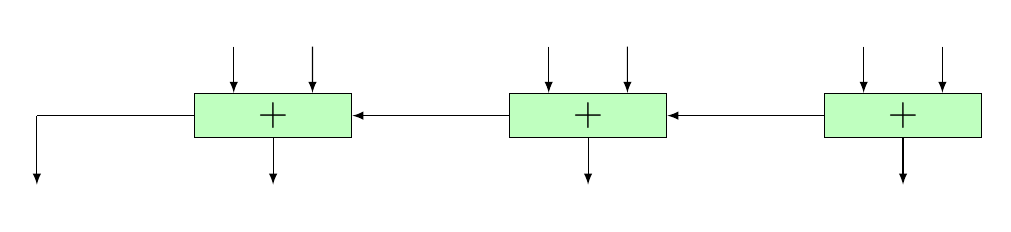
\begin{tikzpicture}

\node[rectangle, draw, fill=green!25, minimum width=2cm] (r0) at (0, 0) {\Large $+$};
\node (x0) at (0.5, 1) {};
\node (y0) at (-0.5, 1) {};
\node (s0) at (0, -1) {};
\draw[-latex] (x0) -- ([xshift=+0.5cm]r0.north);
\draw[-latex] (y0) -- ([xshift=-0.5cm]r0.north);
\draw[-latex] (r0.south) -- (s0);

\node[rectangle, draw, fill=green!25, minimum width=2cm] (r1) at (-4, 0) {\Large $+$};
\node (x1) at (-3.5, 1) {};
\node (y1) at (-4.5, 1) {};
\node (s1) at (-4, -1) {};
\draw[-latex] (x1) -- ([xshift=+0.5cm]r1.north);
\draw[-latex] (y1) -- ([xshift=-0.5cm]r1.north);
\draw[-latex] (r1.south) -- (s1);

\draw[-latex] (r0.west) -- node[above] {} (r1.east);

\node[rectangle, draw, fill=green!25, minimum width=2cm] (r2) at (-8, 0) {\Large $+$};
\node (x2) at (-7.5, 1) {};
\node (y2) at (-8.5, 1) {};
\node (s2) at (-8, -1) {};
\draw[-latex] (x2) -- ([xshift=+0.5cm]r2.north);
\draw[-latex] (y2) -- ([xshift=-0.5cm]r2.north);
\draw[-latex] (r2.south) -- (s2);

\draw[-latex] (r1.west) -- node[above] {} (r2.east);

\node (tmp) at (-11, 0) {};
\node (s3) at (-11, -1) {};

\draw (r2.west) -- node[above] {} (tmp.center);
\draw[-latex] (tmp.center) -- (s3);

\end{tikzpicture}
\end{adjustbox}

\end{minipage}
\end{figure}

%\begin{figure}[htb]
%\centering
%\begin{tikzpicture}
%
%\node[rectangle, draw, fill=green!25, minimum width=2cm] (r0) at (0, 0) {\Large $+$};
%\node (x0) at (0.5, 1) {$x_0$};
%\node (y0) at (-0.5, 1) {$y_0$};
%\node (s0) at (0, -1) {$s_0$};
%\draw[-latex] (x0) -- ([xshift=+0.5cm]r0.north);
%\draw[-latex] (y0) -- ([xshift=-0.5cm]r0.north);
%\draw[-latex] (r0.south) -- (s0);
%
%\node[rectangle, draw, fill=green!25, minimum width=2cm] (r1) at (-4, 0) {\Large $+$};
%\node (x1) at (-3.5, 1) {$x_1$};
%\node (y1) at (-4.5, 1) {$y_1$};
%\node (s1) at (-4, -1) {$s_1$};
%\draw[-latex] (x1) -- ([xshift=+0.5cm]r1.north);
%\draw[-latex] (y1) -- ([xshift=-0.5cm]r1.north);
%\draw[-latex] (r1.south) -- (s1);
%
%\draw[-latex] (r0.west) -- node[above] {$c_0$} (r1.east);
%
%\node[rectangle, draw, fill=green!25, minimum width=2cm] (r2) at (-8, 0) {\Large $+$};
%\node (x2) at (-7.5, 1) {$x_2$};
%\node (y2) at (-8.5, 1) {$y_2$};
%\node (s2) at (-8, -1) {$s_2$};
%\draw[-latex] (x2) -- ([xshift=+0.5cm]r2.north);
%\draw[-latex] (y2) -- ([xshift=-0.5cm]r2.north);
%\draw[-latex] (r2.south) -- (s2);
%
%\draw[-latex] (r1.west) -- node[above] {$c_1$} (r2.east);
%
%\node (tmp) at (-11, 0) {};
%\node (s3) at (-11, -1) {$s_3$};
%
%\draw (r2.west) -- node[above] {$c_2$} (tmp.center);
%\draw[-latex] (tmp.center) -- (s3);
%
%\end{tikzpicture}
%\end{figure}
\end{exercise}

\vspace{-0.5cm}

\begin{exercise}
\begin{enumerate}
\item Wie können wir die Subtraktion zweier Dezimalzahlen durch eine Addition ausdrücken?

\fillwithgrid	{0.5in}

\item Wie können wir die Multiplikation zweier Dezimalzahlen durch Addition\textbf{en} ausdrücken?

\fillwithgrid	{\stretch{1}}

\end{enumerate}
\end{exercise}